\documentclass{report}
\usepackage{hyperref}
\usepackage{graphicx} 
\usepackage{float} 
\usepackage{subfigure} 
\usepackage{booktabs}
\usepackage{diagbox}
\usepackage{amsmath}
\usepackage{bm}
 \usepackage{indentfirst} 
\begin{document}
\renewcommand{\thesection}{\arabic{section}}
\title{Multivariate Time Series Analysis Homeproject}
\author{Bailan He 12118403}
\maketitle
% This will generate a table of contents
\tableofcontents
\newpage 

\section{Data preparation and motivation  (Assignment 1,d) [code line:20 to 66] }
The three indicators used in this article are \textbf{GDP},\textbf{CPI} and \textbf{Unemployment Rate}, downloaded at \url{https://fred.stlouisfed.org/series}. In order to maintain the timeliness and consistency of the data, and to obtain as much data as possible, I use quarterly data from 2000 to 2020, a total of 82 time points. There is no missing value.

I am a novice in the field of economics. I know that GDP, unemployment rate, and CPI are very important macro indicators. And GDP can reflect a more comprehensive macroeconomic. I want to explore whether a VAR model can be constructed between these three variables, and try to analyze the causal relationship between the three indicators.

\section{Data description (Assignment 1,d) [code line:69 to 91]}
In order to put the three indicators in a figure properly, I changed the unit of GDP value to billion and divided the value of CPI by 10. The data obtained is shown as follows:

\begin{figure}[H] 
\centering
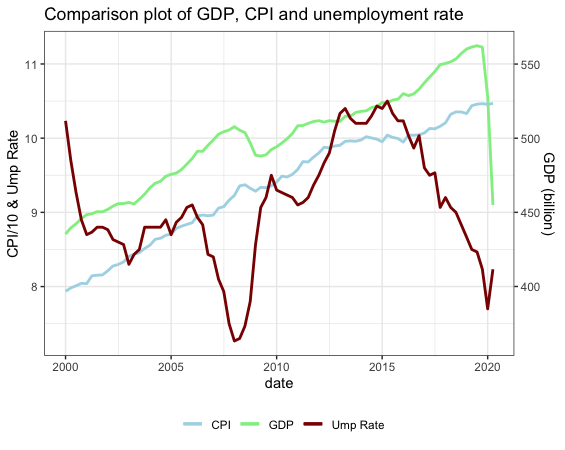
\includegraphics[width=1\textwidth,height=0.4\textheight]{data_plot} 
\caption{Comparison plot of GDP, CPI and unemployment rate} 
\label{Fig.main1}
\end{figure}

Gross domestic product (GDP): a monetary measure of the market value of all the final goods and services produced. (source from: Eurostat). In the Figure \ref{Fig.main1} above, the green line represents GDP, and the Y-axis on the right represents the value of GDP, and its unit is billion. We can see that with the growth of time, France's GDP has also shown a growth trend, but in 2020, due to the Coronavirus, France's GDP has dropped significantly in the two quarters of 2020. Due to the Coronavirus caused a decline in GDP in the two quarters of 2020, resulting in a "fake weak stationary" of GDP.  In the stationarity test, I find that if we do not exclude the two quarters of 2020 data, the result of the test will show that the France's GDP data is weak stationary, which is not consistent with our experience. \textbf{So I think these two data are outliers, when we do the stationarity test, we should exclude the two data in 2020, and we should also exclude the two data when building the model, but when making predictions, we should add these two data to see if our model can predict the impact of coronavirus }.

Consumer price index (CPI): a measure of  changes in the price level of a weighted average market basket of consumer goods and services purchased by households. In the Figure \ref{Fig.main1} above, the lightblue line represents CPI. In order to display the three indicators reasonably, divide the CPI data by 10 here, and the Y-axis on the left represents the value of CPI/10. We can find that France’s CPI has gradually increased over time. Due to the Coronavirus, in the two quarters of 2020, France’s CPI has stopped growing and maintained a stable trend.

Unemployment rate: the number of unemployed people as a percentage of the labour force. In the Figure \ref{Fig.main1} above, the darkred line represents unemployment rate. The Unemployment rate fluctuates over time. The unemployment rate in 2020 is also increasing due to the Coronavirus, although it has shown a downward trend in the previous 5 years.




\section{Stationarity test (Assignment 2, a) [code line:93 to 145]}

Before building the VAR model, we need to check whether the time series are stationary. If the time series is not stationary, we can \textbf{differentiate the data to get the stationary time series}. As I mentioned earlier, due to Coronavirus, the GDP data in the first two quarters of 2020 has experienced a sharp decline, resulting in the result of the GDP data obtained in the ADF test as stationary. So when doing the unit root test here, I did not add the two data for 2020, the total data for each indicator is 82-2=80. Here I use two unit root test methods: use \textbf{adfTest}	 in the \textbf{fUnitRoots} package for ADF test, and \textbf{ur.kpss} in \textbf{urca} package for KPSS test. And I summarize the results as follows:


\begin{table}[H]
\centering
 \caption{\label{tab:original test} Stationarity Tests of Original Data}
 \begin{tabular}{ccccc}
  \toprule
  Time series & GDP(full data)& GDP(removed) & CPI & Ump.rate \\
  \midrule
ADF P-value & 0.01 & 0.99 & 0.99 &0.4752 \\
ADF results & Stationary & Not& Not &Not\\
KPSS statistic & 1.8828&1.9788 &2.1093&0.5004 \\
KPSS results & Not & Not & Not & Not (5pct level)\\
  \bottomrule
 \end{tabular}
\end{table}

From the Table \ref{tab:original test} I find, the ADF test is invalid in the full data of GDP, but when we delete the GDP data for the first two quarters of 2020, the ADF test got the same result as the KPSS test. In this case, KPSS is not affected by violently fluctuating GDP data, and the test maintains consistency. 


Taking into account the economic interpretation, after excluding the data for the two quarters of 2020, I am here not to differentiate the GDP and CPI data, but to convert them into a growth rate to obtain stationary time series. And I make a first-order difference in the unemployment rate to get a stationary unemployment change rate. Results are summarized as follows:


\begin{table}[H]
\centering
 \caption{\label{tab:ratio test} Stationarity Tests of Ratio Data}
 \begin{tabular}{cccc}
  \toprule
  Time series & GDP growth rate & CPI growth rate& Ump.change.rate \\
  \midrule
ADF P-value & 0.01 & 0.01  & 0.01  \\
ADF results & Stationary & Stationary& Stationary\\
KPSS statistic & 0.1121&0.5479 &0.1677 \\
KPSS results & Stationary(10pct) & Stationary(2.5pct) & Stationary(10pct) \\
  \bottomrule
 \end{tabular}
\end{table}

Now all three time series are stationary. I draw a figure to show them.

\begin{figure}[H] 
\centering
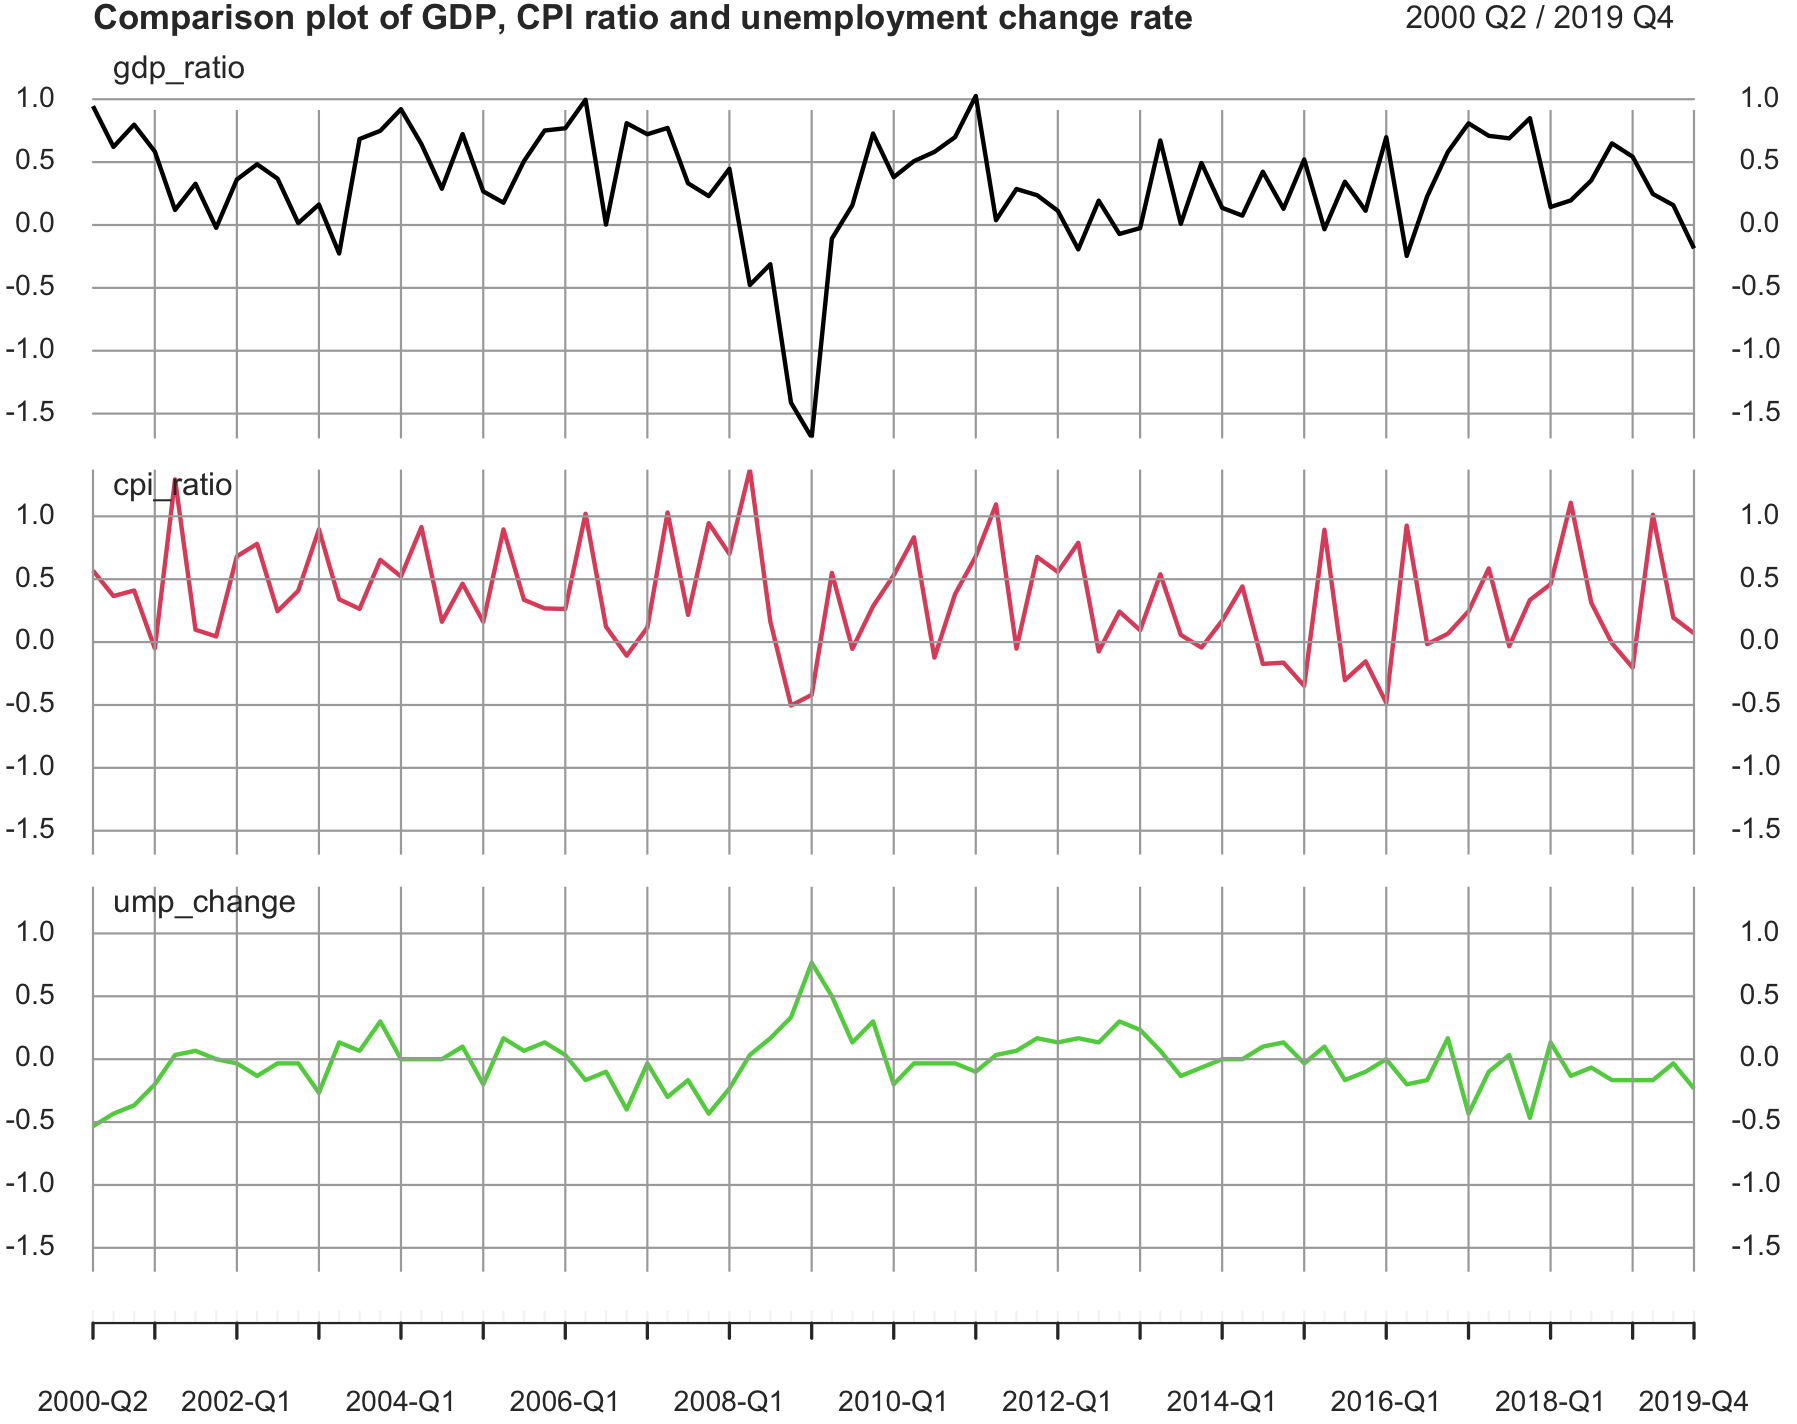
\includegraphics[width=1\textwidth]{ratio_plot} 
\caption{Comparison plot of GDP, CPI ratio and unemployment change rate} 
\label{Fig.main2}
\end{figure}

From the Figure \ref{Fig.main2}, we can find all the  three time series have fluctuating trends and are stationary time series.




\section{ACF Plots ( Assignment 2,b) [code line:147 to 154]}
I use the R basic function \textbf{acf} to draw the ACF Plots of the original and Ratio data:
\begin{figure}[H]
\centering  %图片全局居中
\subfigure[ACF GDP]{
\label{Fig.sub.1}
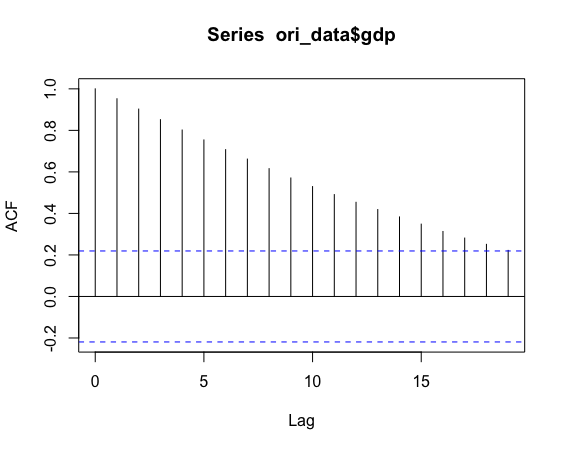
\includegraphics[width=0.45\textwidth]{acf_ori_gdp}}
\subfigure[ACF GDP Ratio]{
\label{Fig.sub.4}
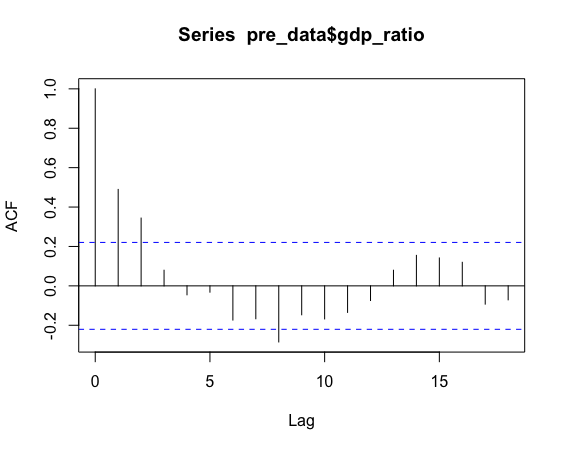
\includegraphics[width=0.45\textwidth]{acf_pre_gdp}}

\subfigure[ACF CPI]{
\label{Fig.sub.2}
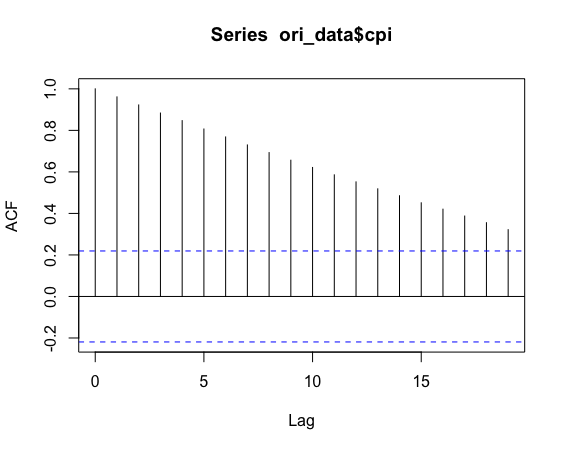
\includegraphics[width=0.45\textwidth]{acf_ori_cpi}}
\subfigure[ACF CPI Ratio]{
\label{Fig.sub.5}
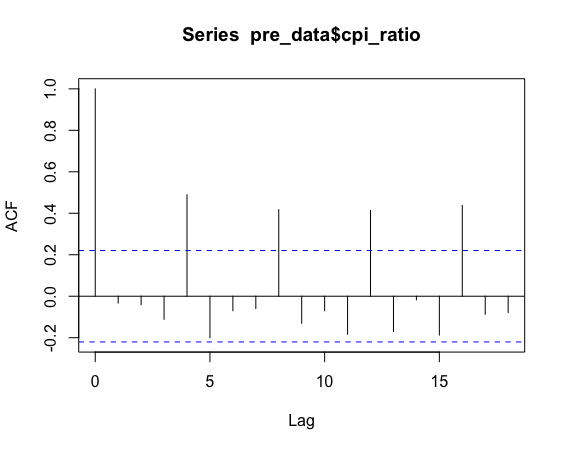
\includegraphics[width=0.45\textwidth]{acf_pre_cpi}}

\subfigure[ACF Ump.Rate]{
\label{Fig.sub.3}
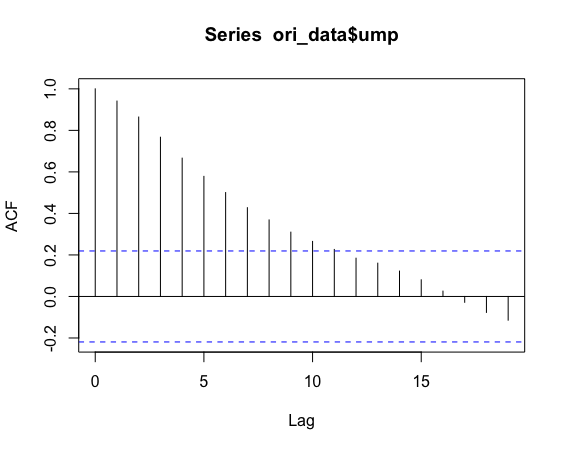
\includegraphics[width=0.45\textwidth]{acf_ori_ump}}
\subfigure[ACF Ump. Change Rate]{
\label{Fig.sub.6}
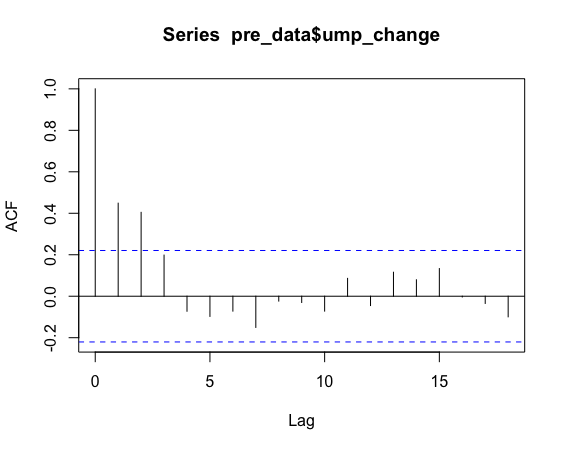
\includegraphics[width=0.45\textwidth]{acf_pre_ump}}
\caption{ACF Plots for the Original and Ratio Data}
\label{Fig.acf}
\end{figure}

In the Figure \ref{Fig.acf}, the three plots on the left column of the figure(a,c,e) represent the autocorrelation function of original data, and all the three autocorrelation functions are statistically significant for lags at least up to 10. This means that the those three indicators are highly correlated with itself. In other words, when the three indicators rise, they tend to continue rising. when they falls, they tend to continue falling. We can reasonably guess that original three time series are not stationary.

The three plots on the right column of the figure(b,d,f) represent the autocorrelation function of Ratio data. As for GDP Ratio(b) and Unemployment change rate(f), their autocorrelation function are statistically significant for lags at most up to 3, which means that the two variable are not highly correlated with each other. Stationarity is a reasonable guess for them.  As for  CPI Ratio, it has obvious seasonal effects, because we can observe that its autocorrelation function is very similar every 4 quarters (that is, a year). When we build the model, we should pay attention to this point. Either the CPI Ratio should be processed in advance and its seasonal factors should be removed, or seasonal factors should be taken into account when building the model. \textbf{In this article, I added dummy variable to consider seasonal factors when building the model}

\section{Cointegration Test [Code line:163 to 166]}

Although we processed the original time series and got the stationary time series, we should check whether there is a cointegration relationship between the variables to determine whether we need to establish a vector error correction model (VECM). \\
I use the function \textbf{ca.jo} of package \textbf{urca} to conducts the \textbf{Johansen procedure}. The result is as follows:

\begin{table}[H]
\centering
 \caption{\label{tab:coin test} Cointegration Test of Ratio Data}
 \begin{tabular}{ccccc}
  \toprule
  Values of teststatistic \\and critical values of test & test& 10pct & 5pct& 1pct \\
  \midrule
r $\leq$ 2 & 15.56 & 6.50&  8.18 &11.65 \\
r $\leq$ 1 & 40.30& 15.66& 17.95 &23.52\\
r = 0  &86.87 &28.71 &31.52 &37.22\\

  \bottomrule
 \end{tabular}
\end{table}

There is clear evidence to reject the all the null hypothesis at the 1\% level and we can likely conclude that there is \textbf{no cointegration relationship } between Ratio Data.

\section{Order Select ( Assignment 2,c) [code line:169 to 178]}

Next, I use the  \textbf{VARselect} function of package \textbf{vars} to select the model order. The \textbf{VARselect} function returns a few different models based on four different information criteria, namely:
 Akaike information criterion (AIC),
Bayesian information criterion (BIC) or Schwarz criterion (SC),
Final Prediction Error (FPE) criterion and 
Hannan–Quinn information criterion (HQC)
When using the AIC criterion, it should be noted that it tends to choose a larger lag order. Therefore, for the VAR model, I prefer to use the BIC criterion. Here, I used \textbf{BIC} as my information criteria.
Earlier we mentioned that because there are seasonal factors in the variable CPI\_Ratio, in addition to choosing the order of the model, I should also choose whether to add seasonal factors.
Based on the above two points, I summarize the results as follows:

\begin{table}[H]
\centering
 \caption{\label{tab:select results} Information Criteria of Model}
 \begin{tabular}{cccccccc}
  \toprule
  \diagbox{Criteria}{Order} &  1     &       2       &     3       &     4       &      5      &       6      &      7\\
  \midrule
AIC(n)& -6.9637& -6.9652& -6.8335& \textbf{-7.1997} & -7.1767 &-7.0547 &-6.8761\\
AIC(n) with season & -7.5403 &\textbf{-7.6151} &-7.4961& -7.4051 &-7.2972& -7.2295& -7.1958\\
HQC(n) & \textbf{-6.8126} &-6.7008& -6.4559 &-6.7088& -6.5724 &-6.3372 &-6.0453\\
HQC(n) with season & \textbf{-7.2760}& -7.2375& -7.0051& -6.8009& -6.5796& -6.3987& -6.2517\\
SC(n)  &\textbf{-6.5842} &-6.3011 &-5.8849 &-5.9665 &-5.6589& -5.2524& -4.7892\\
SC(n) with season  &\textbf{-6.8763}& -6.6665& -6.2629& -5.8874& -5.4948& -5.1426 &-4.8243\\
FPE(n) & 0.0009 & 0.0009  &0.0011&  \textbf{0.0008 } &0.0008&  0.0009 & 0.0011\\
FPE(n) with season & 0.0005&  \textbf{0.0005}&  0.0006&  0.0006&  0.0007 & 0.0008&  0.0008\\
 \bottomrule
 \end{tabular}
\end{table}

In the Table \ref{tab:select results} above, I bolded the information criteria value corresponding to the best order. I found that after adding seasonal factors, the information criteria value of the model with the same order is significantly lower, which means the model fits better. So in the end I chose the \textbf{VAR(1) model with seasonal dummy variables}, it has the lowest BIC as -6.8763.

\section{Train VAR(1) ( Assignment 2,d) [code line:179 to 185]}

Before training the model, I first divide the data into a training set and a test set. As mentioned earlier, the data for the first two quarters of 2020 has changed significantly due to Coronavirus compared to other data. It is like a black swan event, and use these data to build model will increase the variance of the model, I think it is inappropriate. So I add them to the test set. On this basis, since my purpose of establishing the VAR model is to predict the changes of the three indicators in the next time, I also add the latest two years of data to the test set. So the test set includes 10 data from 2018 to 2020, and the remaining data is used as the training set. It is worth noting that because I performed the difference, the total data for the first quarter of 2000 was lost, and my total data was reduced from 82 to 81. In summary, \textbf{I use a total of 71 data from the second quarter of 2000 to the fourth quarter of 2017 as the training set, and use a total of 10 data from the first quarter of 2018 to the second quarter of 2020 as the test set}.

Then I use \textbf{VAR} function of package \textbf{vars} to build VAR(1) with 4 levels seasonal dummy variable .  Let  $\bm{Y}=(GDP.Ratio,CPI.Ratio,Ump.Change\ Rate)^{\mathrm{T}}$, using \textbf{OLS method} to get the VAR(1) model:

\begin{equation*}%加*表示不对公式编号
\begin{split}
\bm{Y_t} = 
\left[ \begin{matrix}
\textbf{0.153} \\
\textbf{0.190} \\
\textbf{0.057}
\end{matrix}\right] +
\left[ \begin{matrix}
\textbf{0.545}&-0.028&0.103\\
\textbf{0.239}&\textbf{0.242}&0.115\\
\textbf{-0.195}&-0.003&\textbf{0.289}
\end{matrix}\right] \bm{Y_{t-1}} +
\left[ \begin{matrix}
-0.149\\
\textbf{0.579}\\
0.077
\end{matrix}\right]season_1 \\ +
\left[ \begin{matrix}
0.005\\
\textbf{-0.314}\\
0.014
\end{matrix}\right]season_2 + 
\left[ \begin{matrix}
-0.004\\
0.027\\
0.048
\end{matrix}\right]season_3 + \bm{\epsilon_t}
\end{split}
\end{equation*}


In the above formula, I use bold numbers to indicate statistically significant coefficients. \textbf{As mentioned in the class, in the reduced form VAR model, the coefficients may not has meaningful
economical interpretation}. But I think statistically valid coefficients can still explain the relationship between variables.

For GDP ratio, only the coefficient of GDP ratio in the last time period is statistically significant, which means that the other two variables and seasonal dummy variables are not statistically significant in predicting GDP ratio. This coefficient 0.545 means that when other variables remain the same, change the GDP growth rate of the previous quarter by 1 percentage, and the GDP growth rate of this quarter will increase by 0.545 percentage.

For the CPI ratio, in addition to the GDP ratio and CPI ratio coefficients of the previous time period, there are also two seasonal dummy variable coefficients that are also statistically significant. It shows that CPI is affected by seasonality, which is consistent with our ACF plot, and GDP ratio will also affect the prediction of CPI ratio. I guess there may be Granger causality between these two variables. And the correlation coefficient here can be explained as above.

For the Unemployment change rate, in addition to its own coefficient of the last time period which is statistically significant, the coefficient of the GDP ratio of the last time period is also statistically significant. It shows that there may be Granger causality between GDP ratio and Unemployment change rate.

\section{Diagnostic Test (Assignment 2,e) [code line:187 to 215]}

After constructing the VAR(1) model, we should also test whether the residuals of the model has serial correlation, whether the residuals are normally distributed and whether the residuals are stable.

Serial correlation: \textbf{it will affect the efficiency of OLS estimators, this leads to the null hypothesis of estimated parameters that may be falsely rejected. And If the residuals obtained in the low-order VAR model have serial correlation, then we should consider increasing the order of the VAR model until the residual sequence obtained does not have serial correlation. This is also a reference index for choosing the order of the model.} So it is necessary to investigate whether the residuals display serial-correlation. Here I use the function \textbf{serial.test} from package \textbf{vars} to do the \textbf{Portmanteau Test}. The value of test statistic $\chi^2=139$ and P-value=0.4, which means the null hypothesis can't be rejected. Therefore, \textbf{there is no serial correlation in our model residuals}.

Normality of the residuals: the VAR model requires the residuals to be normally distributed, so we should also test the normality of the residuals. At the beginning, I used the function \textbf{normality.test} of package \textbf{vars} for normality test, but  the normality hypothesis of the residuals for my VAR(1) model is rejected. I think this is because my sample size is not large enough, so the Jarque Bera test will almost always reject normality of the residuals for my VAR model. Then I directly draw the Q-Q plots.

\begin{figure}[H]
\centering  %图片全局居中
\subfigure[Residual GDP\_Ratio]{
\label{Fig.sub.7}
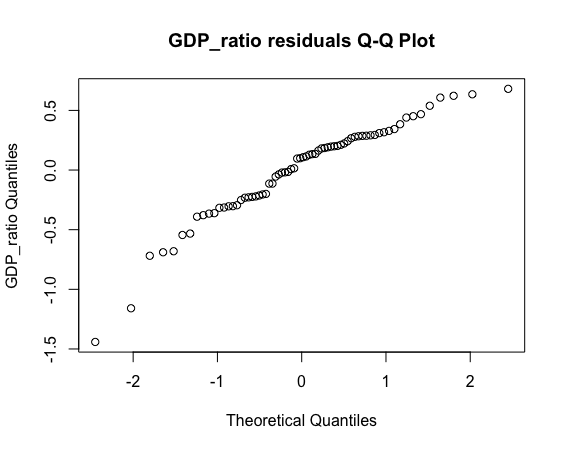
\includegraphics[width=0.3\textwidth]{qq_gdp}}
\subfigure[Residual CPI\_Ratio]{
\label{Fig.sub.8}
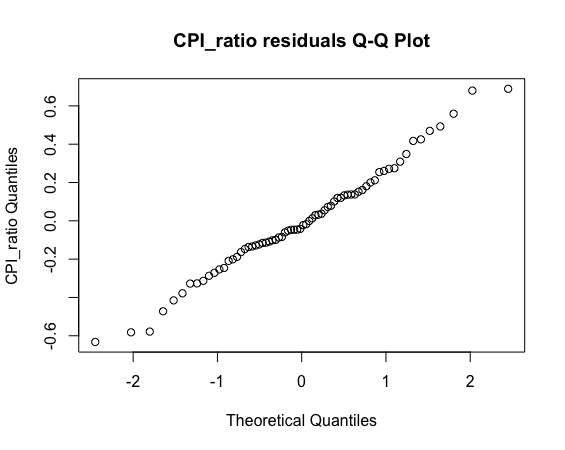
\includegraphics[width=0.3\textwidth]{qq_cpi}}
\subfigure[Residual Ump.change]{
\label{Fig.sub.9}
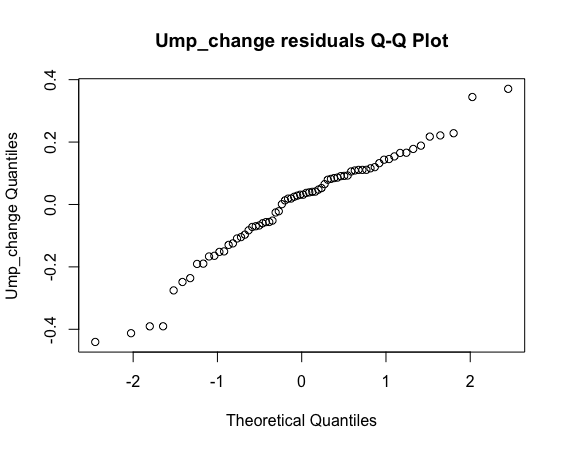
\includegraphics[width=0.3\textwidth]{qq_ump}}
\caption{Residual Q-Q plots}
\label{fig.qq}
\end{figure}

In the Figure \ref{fig.qq}, I find that the residual of GDP growth rate deviates slightly from normal distribution, but the residuals of CPI growth rate and Ump. change basically conformed to the normal distribution.

Test for System stability:  I use the function \textbf{stability} of package \textbf{vars} to test the model stability.

In the Figure \ref{Fig.stab}, the cumulative sum of residuals curve takes time as the abscissa. Two critical lines are drawn in the figure. If the cumulative sum exceeds these two critical lines, the parameters are not stable. It can be seen that the model is stable.

\begin{figure}[H] 
\centering
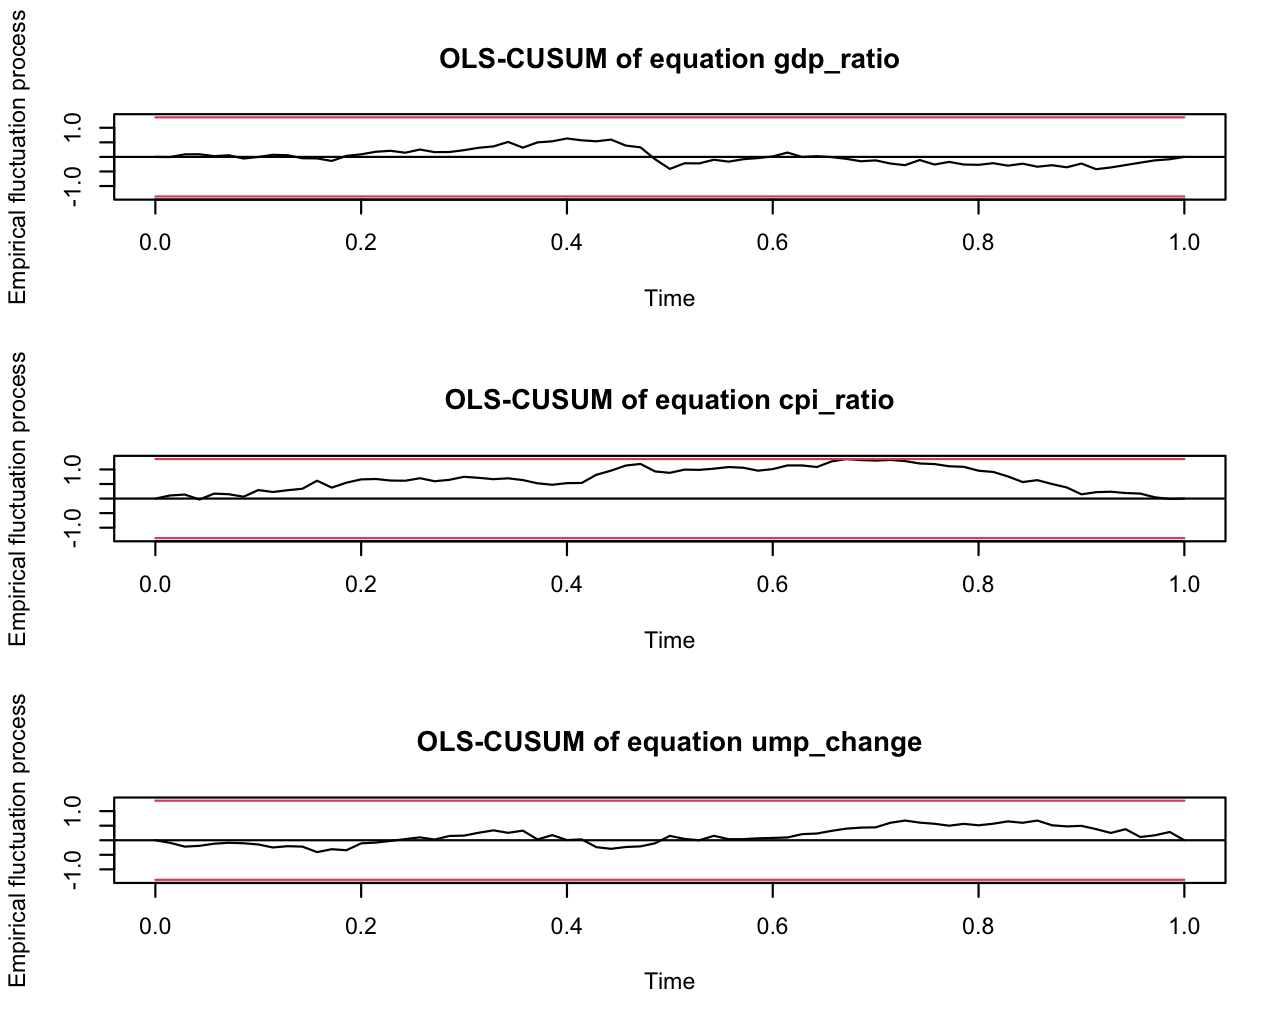
\includegraphics[width=1\textwidth]{var_stab} 
\caption{ System stability} 
\label{Fig.stab}
\end{figure}

As requested, I draw residual plots of three variables. It can be seen that, except for the residuals of GDP growth rate that fluctuate violently in the intermediate samples, the remaining residuals seem to be relatively stable, indicating that the model setting is relatively reasonable.

\begin{figure}[H] 
\centering
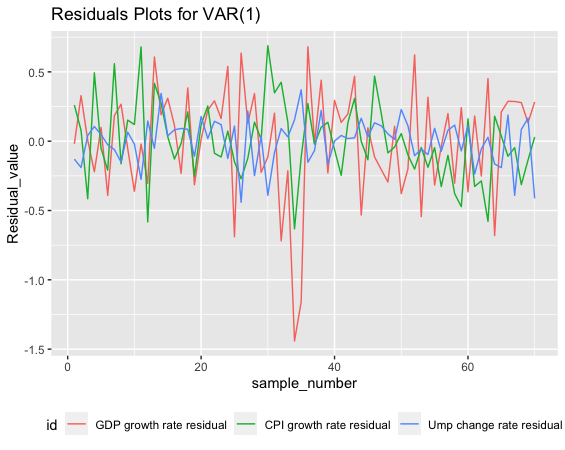
\includegraphics[width=1\textwidth]{var_residual} 
\caption{VAR(1) residual plot} 
\label{Fig.residual}
\end{figure}


\section{One-step and Three-step Forecast (Assignment 2,f) [code line:220 to 311]}

I use function \textbf{predict} of package \textbf{vars} to do a one-step and a three-step forecast, and draw a line graph of the forecast value and the true value of every variable. In addition, I also draw a line graph of the square error between one-step prediction and three-step prediction and the true value of every variable to evaluate predictions.

\begin{figure}[H]
\centering  %图片全局居中
\subfigure[Forecast for GDP growth ratio]{
\label{Fig.sub.10}
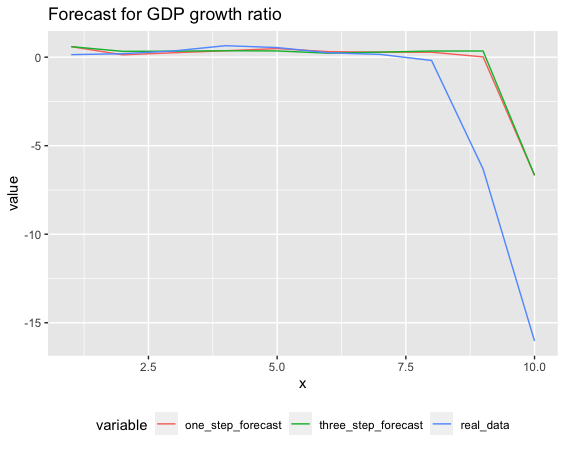
\includegraphics[width=0.45\textwidth]{forecast_gdp}}
\subfigure[Square error for GDP growth ratio]{
\label{Fig.sub.11}
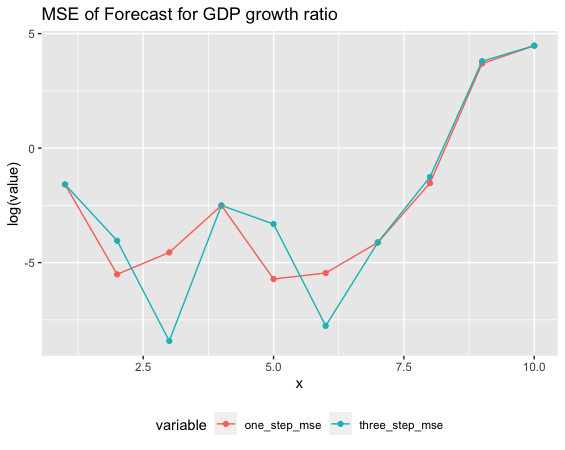
\includegraphics[width=0.45\textwidth]{mse_gdp}}

\subfigure[Forecast for CPI growth ratio]{
\label{Fig.sub.12}
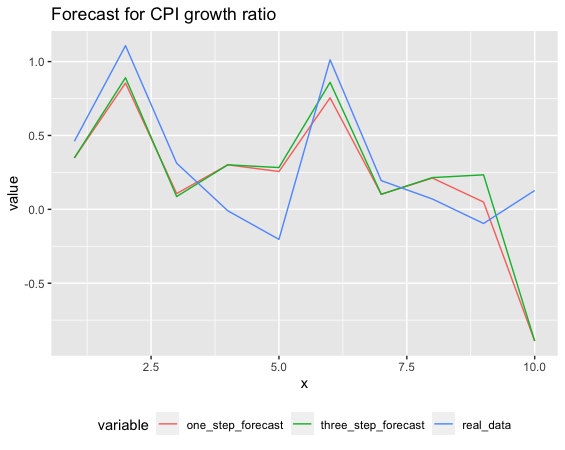
\includegraphics[width=0.45\textwidth]{forecast_cpi}}
\subfigure[Square error for CPI growth ratio]{
\label{Fig.sub.13}
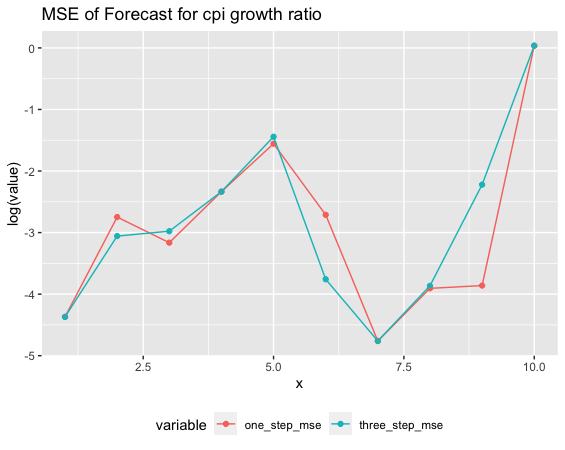
\includegraphics[width=0.45\textwidth]{mse_cpi}}

\subfigure[Forecast for Ump. change rate]{
\label{Fig.sub.14}
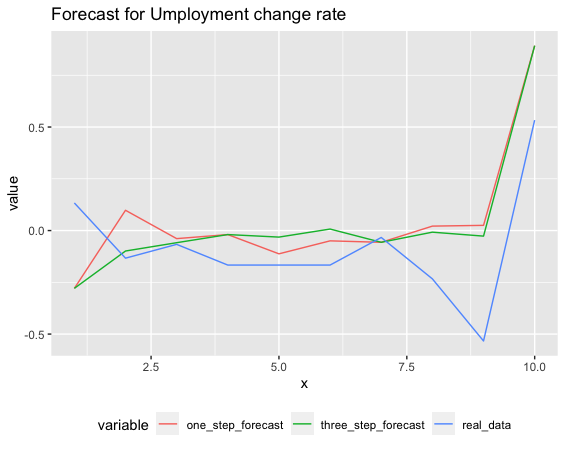
\includegraphics[width=0.45\textwidth]{forecast_ump}}
\subfigure[Square error for Ump. Change Rate]{
\label{Fig.sub.15}
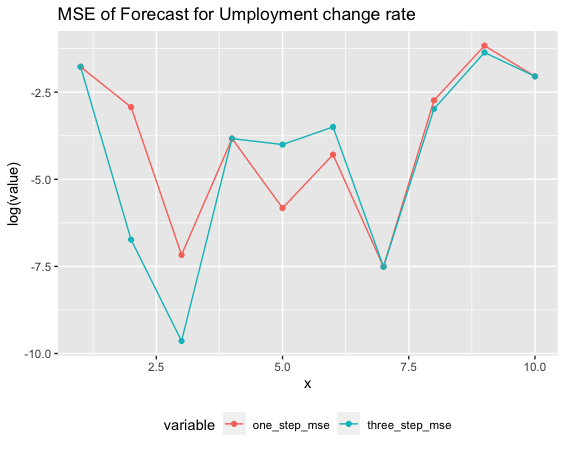
\includegraphics[width=0.45\textwidth]{mse_ump}}
\caption{One-step and Three-step Forecast and Square error}
\label{Fig.forecast}
\end{figure}

In the Figure \ref{Fig.forecast}, the three plots in the left column represent the comparison of one-step prediction and three-step prediction with the true value and the three plots in the right column represent the square error of one-step prediction and three-step prediction from the true value. It should be noted that in order to better show the difference between the one-step forecasts and the three-step forecasts error in the figure, I have performed \textbf{log processing on the square error} here. The MSE of one-step forecast is 13.056, and the MSE of three-step forecast is 13.495. So the one-step forecast seems better.

Regarding the GDP growth rate, it is obvious that due to coronavirus, France’s GDP growth rate in the two quarters of 2020 has experienced a sharp decline, resulting in very inaccurate model forecasts and very large errors. For the 8 data from 2018 to 2019, the overall error is not big, and the interesting thing is that when comparing the one-step forecast and the three-step forecast, I found that the forecast of the second step of each three-step forecast is worse than corresponding one-step forecast (Corresponding to the x coordinate 2 and 5 in plot (b), the red line is below the green line), but the forecast of the third step of each three-step forecast is better than corresponding one-step forecast (Corresponding to the x coordinate 3 and 6 in plot (b), the red line is higher the green line).It shows that when the model predicts GDP growth rate, it is more accurate in the long-term forecast than in the short-range forecast.

For the forecast of CPI growth rate, there is little difference between the one-step forecast and the three-step forecast as a whole, but we can see from plot (d) that for the forecast of the CPI growth rate in 2019, the one-step forecast is better, for after 2019 the three-step forecast of CPI growth rate is better. We can also see that France’s CPI growth rate has also been abnormal due to coronavirus, which has led to a sudden increase in forecast errors.

For the unemployment change rate, it can be seen from plot (f) that the three-step forecast is better in 2018, but the one-step forecast is better in 2019. It is worth noting that the unemployment rate in France has a significant decline in the first quarter of 2020. Neither type of forecasts predicted this decline. With the impact of the coronavirus, the unemployment rate in France rose again in the second quarter of 2020, and the model also does not predict this.

Forecasts are usually not precise enough to be all that informative from a practical standpoint. Instead, in practice we will usually end up looking at the following three things that are derived from the fitted VAR model: Granger Causality, Impulse Response Functions, and Forecast Error Variance Decomposition.

\section{Granger-Causality test(Assignment 3, a) [code line:314 to 343]}

I use function \textbf{grangertest} of package \textbf{lmtest} to see if the the three indicators influence each other. The results of the test are summarized in the following table:

\begin{table}[H]
\centering
 \caption{\label{tab:gc} Granger-Causality test results}
 \begin{tabular}{ccccc}
  \toprule
\textbf{H1} & P-value & whether granger cause \\
  \midrule
GDP g.r. granger cause CPI g.r. & 0.008  & Yes\\
CPI g.r granger cause GDP g.r. & 0.976 & No\\
Ump. c.r granger cause GDP g.r & 0.471 & No \\
GDP g.r granger cause Ump. c.r & 0.0003 & Yes\\
CPI g.r. granger cause Ump. c.r & 0.615 & No\\
Ump. c.r granger cause CPI g.r. & 0.214 & No\\
  \bottomrule
 \end{tabular}
\end{table}

From the results in the Table \ref{tab:gc}, I draw the following conclusions:

1. GDP growth ratio  Granger causes CPI growth ratio, which means past values of GDP growth ratio  improve prediction of CPI growth ratio (compared to only past values of CPI growth ratio). In other words, exclusion of past values of GDP growth ratio, the information set should enlarge the MSE of the forecast of CPI growth ratio.
But on the contrary, CPI growth ratio do not Granger cause GDP growth ratio. The inclusion of present and past realizations of CPI growth ratio in the information set does not affect the MSE of forecast of GDP growth ratio.

2. GDP growth ratio  Granger causes Unemployment change rate, which means past values of GDP growth ratio  improve prediction of Unemployment change rate (compared to only past values of Unemployment change rate). In other words, exclusion of past values of GDP growth ratio, the information set should enlarge the MSE of the forecast of Unemployment change rate
But on the contrary, Unemployment change rate, does not Granger cause GDP growth ratio.
The inclusion of present and past realizations of Unemployment change rate in the information set does not affect the MSE of any h-steps-ahead forecast of GDP growth ratio.

3. There is no Granger causality between Unemployment change rate and CPI growth ratio.

4. There is no feedback system, because no sub-processes of the VAR process Granger-cause each other.

The function \textbf{causality} in the \textbf{vars} package can test Granger causality after building the model. I summarize the results as follows:

\begin{table}[H]
\centering
 \caption{\label{tab:gc2} Granger-Causality test results after building VAR model}
 \begin{tabular}{ccccc}
  \toprule
\textbf{H1} & P-value & Conclusion\\
  \midrule
GDP g.r. granger cause CPI g.r. and Ump. c.r & \textless 2.2e-16  & Yes\\
\\
Instantaneous causality between \\GDP g.r. and CPI g.r. + Ump. c.r  & 0.02 & Yes\\
\\

CPI g.r granger cause GDP g.r. and Ump. c.r & 0.99 & No\\
\\
Instantaneous causality between \\CPI g.r. and GDP g.r. + Ump. c.rr & 0.4252 & No\\
\\
Ump. c.r granger cause GDP g.r and CPI g.r.  & 0.72 & No \\
\\
Instantaneous causality between \\ Ump. c.r and GDP g.r and CPI g.r. & 0.016 & Yes\\
  \bottomrule
 \end{tabular}
\end{table}

From the results in the Table \ref{tab:gc2}, I can draw the following conclusions:

1. GDP growth ratio Granger causes the sub-process CPI growth ratio and Unemployment change rate.

2. CPI growth ratio and Unemployment change rate does not Granger cause corresponding the rest sub-process.

3. There is instantaneous causality between GDP growth ratio and (CPI growth ratio, Unemployment change rate).

4. There is instantaneous causality between Unemployment change rate and (CPI growth ratio, GDP growth ratio).

The results of Granger causality above are consistent with my knowledge of economics. In my opinion, GDP is an important comprehensive macro index, so the GDP growth rate should include the information of CPi growth rate and unemployment rate. Therefore, the GDP growth rate will have Granger causality for the CPI growth rate and the unemployment rate. On the contrary, because GDP is a very comprehensive indicator, it already contains a lot of information, including the information of CPI growth rate and unemployment rate. Therefore, neither the CPI growth rate nor the unemployment rate has the Granger causality for the GDP growth rate. And there is no direct causal relationship between the CPI growth rate and the unemployment rate. Granger causality test also confirms this result.

\section{Impulse-Response Analysis(Assignment 3, b) [code line:345 to 347]}

By using function \textbf{irf} in the package \textbf{vars}, The Impulse-Response plot corresponding to each variable is as follows:

\begin{figure}[H]
\centering  %图片全局居中
\subfigure[Impulse-Response for GDP g.r. ]{
\label{Fig.sub.16}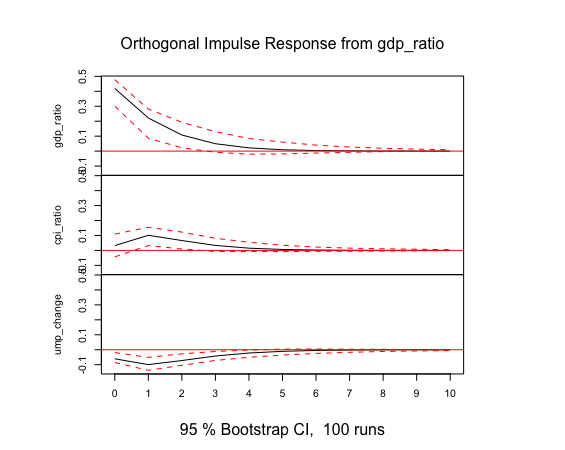
\includegraphics[width=0.48\textwidth]{irf_1}}
\subfigure[Impulse-Response for CPI g.r. ]{
\label{Fig.sub.17}
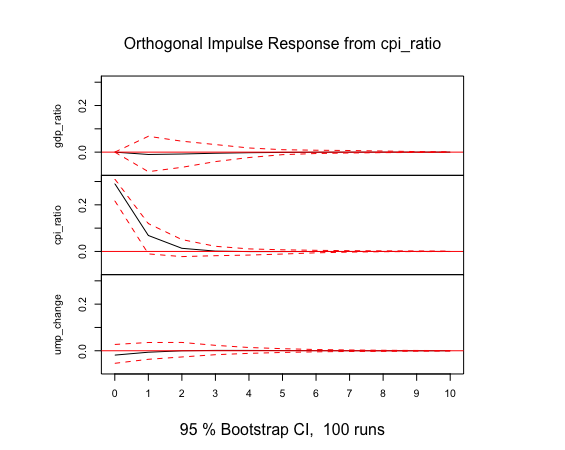
\includegraphics[width=0.48\textwidth]{irf_2}}

\subfigure[Impulse-Response for Ump. change rate]{
\label{Fig.sub.18}
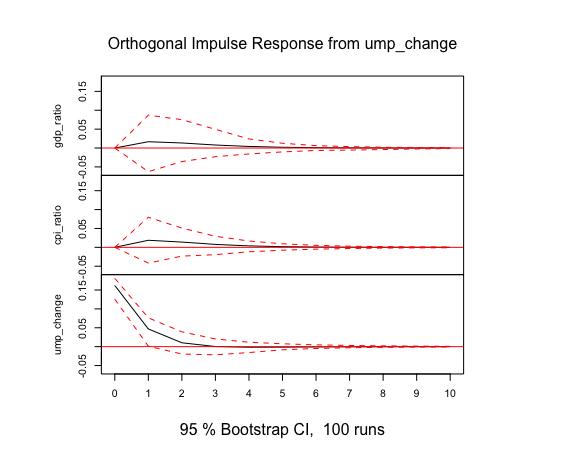
\includegraphics[width=0.48\textwidth]{irf_3}}
\caption{Impulse-Response Analysis for VAR(1)} 
\label{Fig.irf}
\end{figure}

From the Figure \ref{Fig.irf} above, my conclusion is as follows:


1. One standard deviation shock to GDP growth ratio causes statistically significant increases on itself for 2 periods, after which the effect dissipates. The increment brought by this shock gradually decreases as the period grows.

2. One standard deviation shock to GDP growth ratio causes statistically significant increases on CPI growth ratio for 2 periods, after which the effect dissipates.  The increase peaks in period 1, ca. 0.1.

3. One standard deviation shock to GDP growth ratio causes statistically significant decreases on Unemployment rate for 3 periods, after which the effect dissipates. The decrement peaks in period 1, ca. -0.1.

4. One standard deviation shock to CPI growth ratio dose not cause statistically significant change on GDP growth ratio.  

5. One standard deviation shock to CPI growth ratio causes nearly statistically significant increases on itself for 2 periods, after which the effect dissipates. The increment brought by this shock gradually decreases as the period grows.

6. One standard deviation shock to CPI growth ratio dose not cause statistically significant change on Unemployment rate.

7. One standard deviation shock to  unemployment rate dose not cause statistically significant change on GDP growth ratio. It can be seen here that the confidence interval formed by bootstrap is very large, and includes positive and negative values. So does not have statistical meaning.

8. One standard deviation shock to  unemployment rate dose not cause statistically significant change on CPI growth ratio.

9. One standard deviation shock to unemployment rate causes statistically significant increases on itself for 1 periods, after which the effect dissipates. The increment brought by this shock gradually decreases as the period grows.

It can be seen from the results of Impulse-Response that the shock of GDP growth rate not only affects itself, but also affects the other two variables in a statistically significant sense, but the CPI growth rate and unemployment rate will only affect itself. Their effects on the remaining variables is not statistically significant. This is highly consistent with the results of our Granger causality test.


\section{Forecast Error Variance Decomposition(Assignment 3, c) [code line:349 to 351]}

In a FEVD, forecast errors are considered for each equation in the fitted VAR model, then the fitted VAR model is used to determine how much of each error realization is coming from unexpected changes (forecast errors) in the other variable. I use the function \textbf{fevd} from the package \textbf{vars} to calculate them and visualize in a plot.

\begin{figure}[H] 
\centering
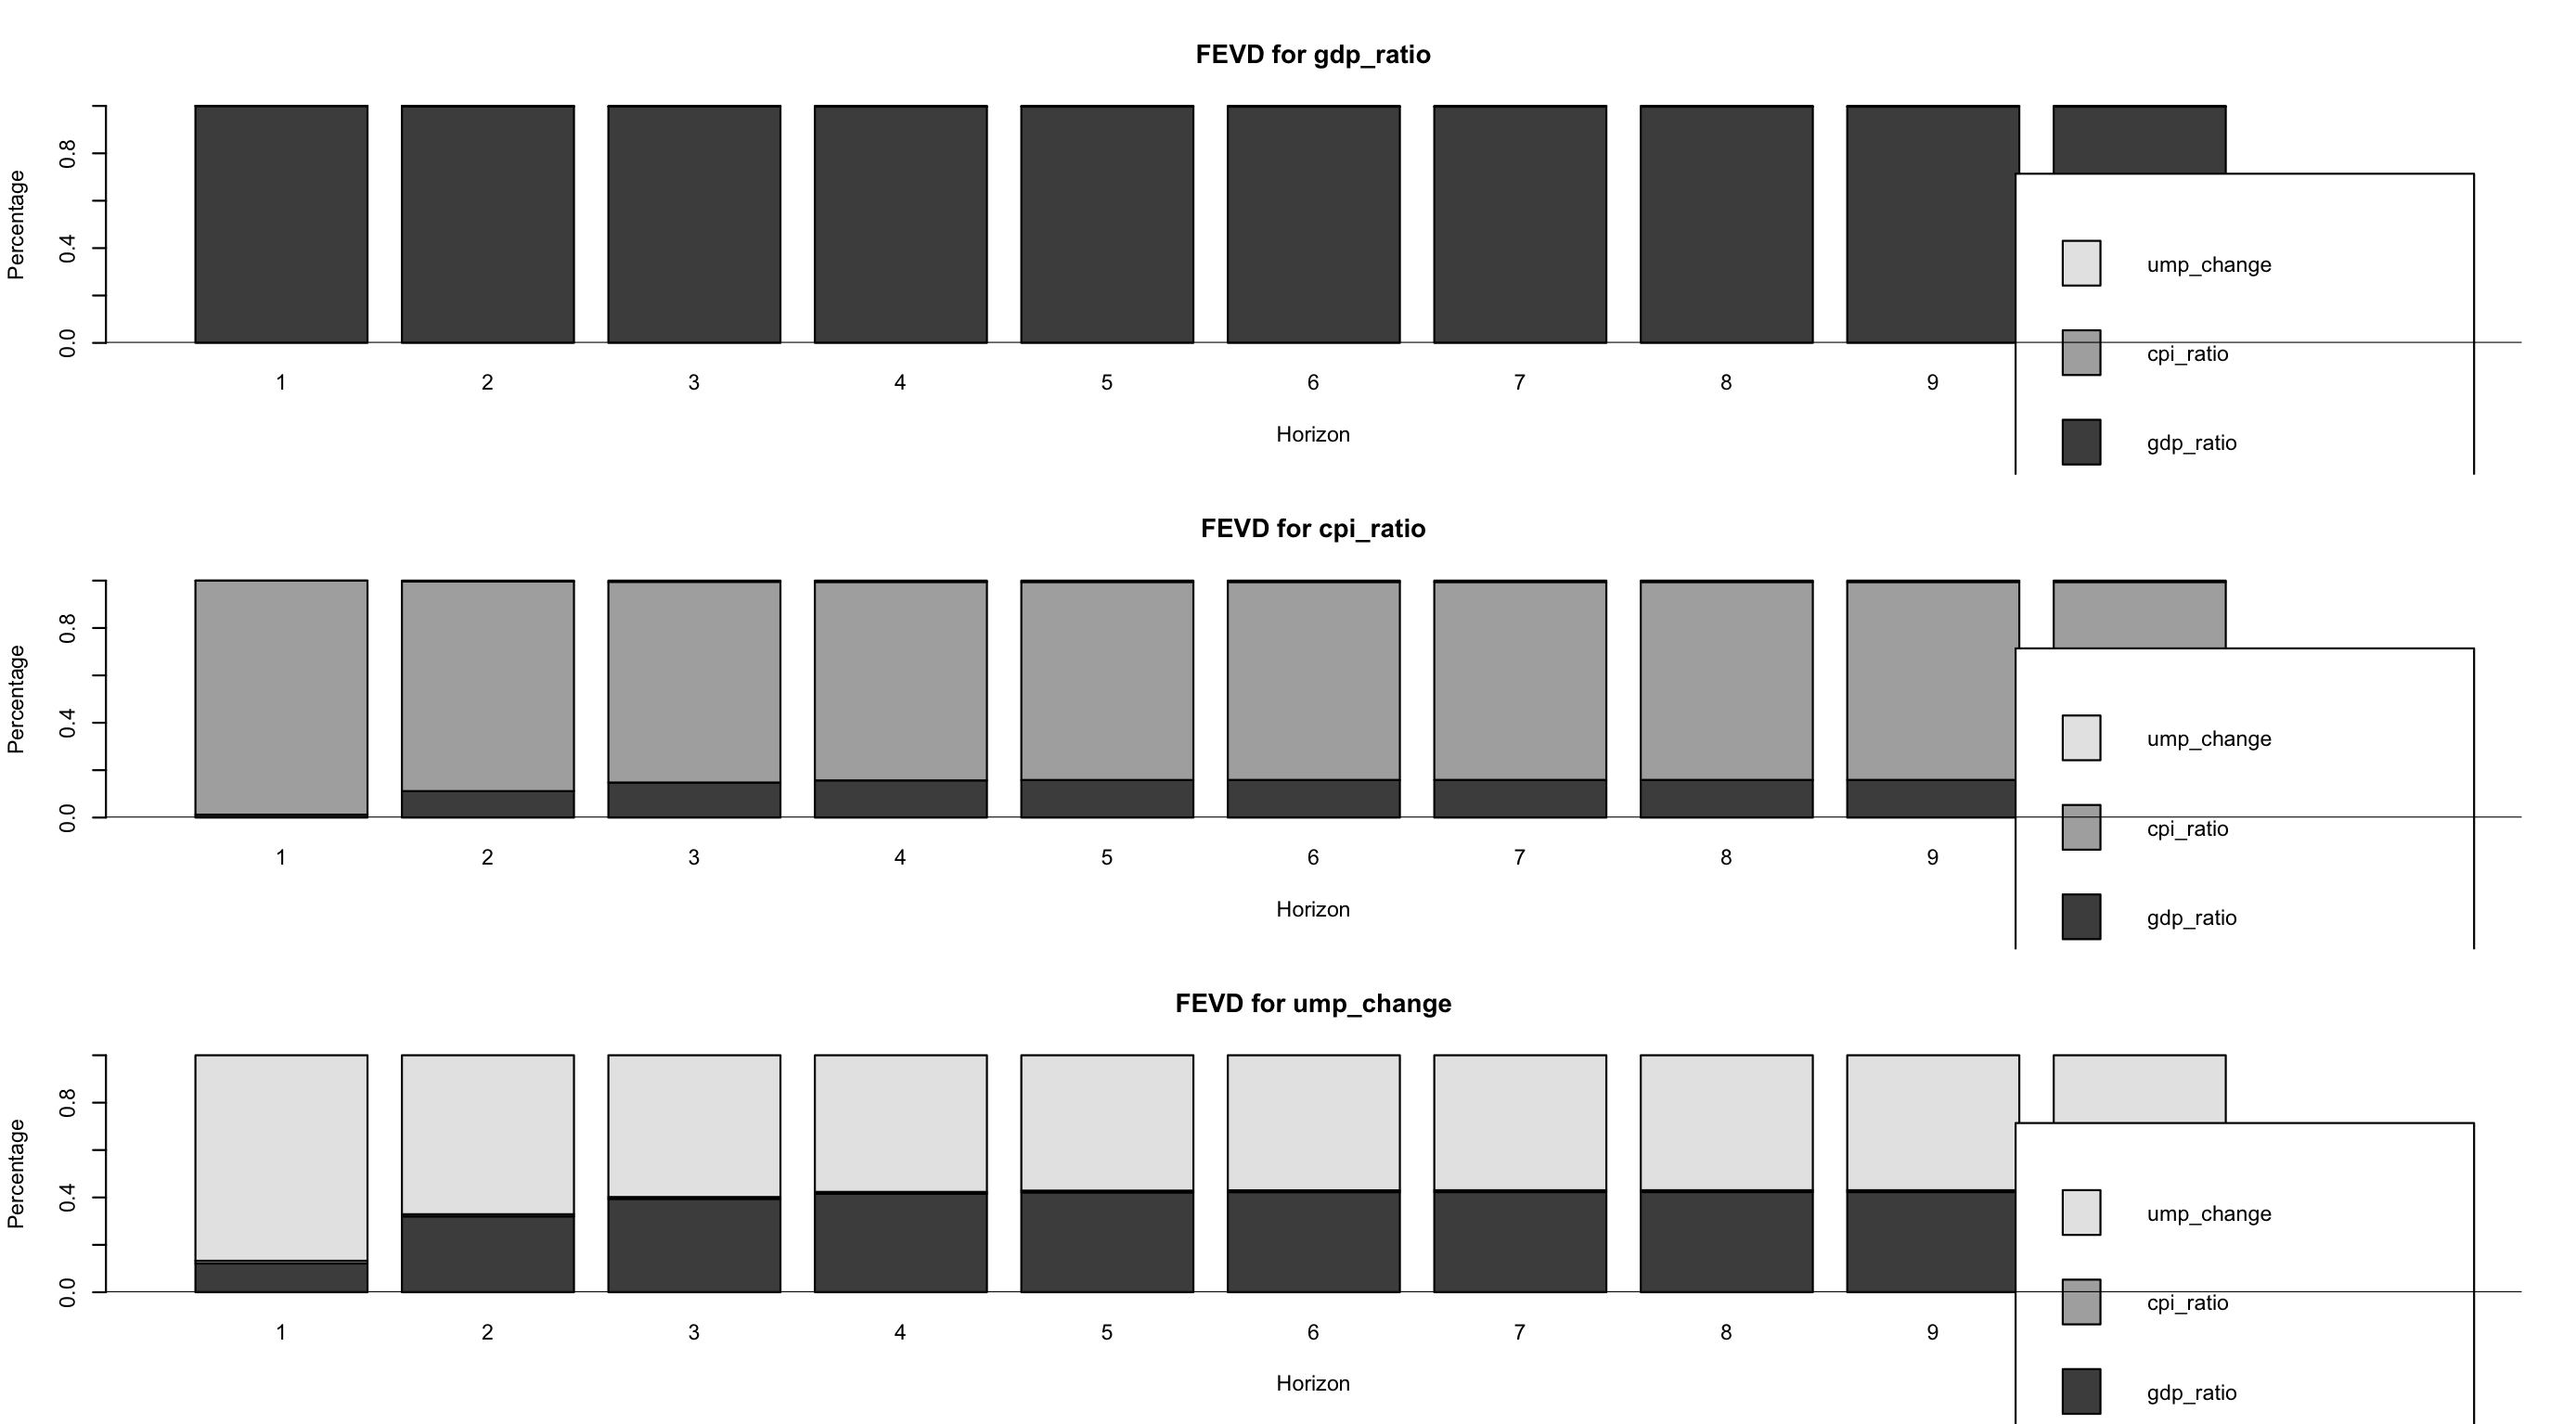
\includegraphics[width=1\textwidth]{fevd} 
\caption{Forecast Error Variance Decomposition for VAR(1)} 
\label{Fig.fevd}
\end{figure}

In the first plot, we see the FEVD for GDP growth ratio. it reveals that magnitude of the causality between GDP growth ratio and other two variable is tiny, we can’t even see the contribution from CPI growth ratio and Unemployment change rate on the FEVD graph.

Conversely, it appears GDP growth ratio account for about 15\% of the forecast error variance in the 
CPI growth ratio equation, and the magnitude of the causality between CPI growth ratio and Unemployment change rate is nearly zero. It is noteworthy that before period 4, the proportion of GDP growth ratio in the forecast error variance increased from 1\% to 15\%, and remained unchanged after period 4.  This shows that for the forecasts of relatively recent period, the CPI growth rate itself accounts for a large proportion, but for the forecasts of relatively distant period, the proportion of GDP growth rate is gradually increasing, because the GDP growth rate reflects the overall economic situation. It is relatively stable and contain some information about the CPI growth rate. Therefore, when predicting the CPI growth rate, the overall economic situation of the previous few years should be taken into account, which is consistent with my economic knowledge.

As for Unemployment change rate, GDP growth ratio account for about 42\% of the forecast error variance in the equation of Unemployment change rate  and the magnitude of the causality between CPI growth ratio and Unemployment change rate is nearly zero. We can notice that, similar to the CPI growth rate, the proportion of the forecast error variance of the GDP growth rate in the unemployment rate also gradually increases with the growth of the period. From the initial 12\% to 42\% and maintain this proportion. In my opinion, the GDP growth rate reflects the overall economic situation, the change in the unemployment rate is highly correlated with the increase or decrease in the GDP growth rate. For example, a high GDP growth rate may represent a decrease in the unemployment rate. Therefore, compared with the CPI growth rate, GDP The percentage of growth rate in this case is better, which is in line with my knowledge of economics.

All the above results are consistent with the results obtained in the Granger causality test.

\end{document}
